\documentclass[12pt,a4paper]{report}

\usepackage[utf8]{inputenc}
\usepackage[english]{babel}
\usepackage[left=2.5cm,right=2.5cm]{geometry}

\usepackage{amsmath}
\usepackage{amsfonts}
\usepackage{amssymb}
\usepackage{graphicx}
\usepackage{multicol}
\usepackage{fancyhdr}
\usepackage{wrapfig}
\usepackage{lipsum}
\usepackage{caption}

\author{S. Bourgeois}


\begin{document}

\bibliographystyle{plain}

\pagestyle{fancy}

\fancyhead{} % clear all header fields
\fancyhead[L]{\small Nuclear energy for space exploration: A technological necessity \\ or a risky gamble for humanity and the wider environment ?}
\fancyhead[R]{\small BOURGEOIS Sacha\\
2025}
\fancyfoot{} % clear all footer fields

\begin{titlepage}
\begin{center}

\textup{\small {\bf First year of Master's Internship} \\ Report}\\[2cm]

% Title
\LARGE \textbf {Nuclear energy for space exploration: \\
A technological necessity or a risky gamble for humanity and the wider environment ?}\\[3cm]



       

% Submitted by
\normalsize Submitted by \\[0.2cm]
\textbf{S. Bourgeois}\\
M1 PFA\\
\vspace{0.5cm}
Under the guidance of\\[0.2cm]
\textbf{S. Porteboeuf-Houssais, J. Donini}\\
Profs.



\vspace{1cm}

% Bottom of the page

\includegraphics[width=0.2\textwidth]{img/UCA-logo.png}\\[0.5cm]
\Large{Department of Physics}\\
\normalsize
\textsc{Université Clermont Auvergne}\\
4 Avenue Blaise Pascal\\
63178 Aubière\\
\vspace{0.2cm}
11th of June 2025

\end{center}

\end{titlepage}
\newpage

\chapter*{Acknowledgment}
\quad Before further development on this work I would like to thank those who have helped to structure and carry it out.\\

First and foremost I would like to thank my tutors Mister Donini and Miss Porteboeuf-Houssais for their involvement and their guidance during this project and this first year of Master's. \\

Then comes the rest of our team, Victor Auga-Bascou, Yael Chahinian and Yvon Marthon with whom I have worked for these pasts eight weeks. I want to thank them for their patience and their teamwork abilities.\\

I also thank Pauline D., Pauline P., Camille D. and Elisa B for proofreading this report, for their hospitality and their unwavering support. \\

Lastly, I thank you, reader of this report, for taking some of your time to understand and grade this work. Without you all of this would be useless.
\newpage
\chapter*{Foreword}

Let us first understand what this work constitutes and how it was structured.\\


For the past two months Victor, Yael, Yvon and I have studied, under the tutoring of Sarah and Julien.
This work we have been doing differs from a "classical" internship in that it was mostly bibliographic until the end whence it differed widely. \\

Indeed, we had a mock-up debate wherein each of us students had to take on different roles and perspectives while trying to answer our research question : "Nuclear energy for space exploration: A technological necessity or a risky gamble for humanity and the wider environment ?".\\
This TER used to be a class centered around "Nuclear energy and Society", taught during the second semester of master's, its objective was to spur students into developing  their ability to communicate and debate around a science-focused subject as well as to lead bibliographic research.\\

Our work differs from those that came before us in that we didn't focus our research on nuclear power plants or atomic weapon proliferation but rather on space exploration and radiation shielding.\\

We hope that you will find this report interesting and perhaps even learn a thing or two along the way.
\newpage

\tableofcontents


\chapter*{Introduction}

% 	states your hypothesis 	explains how you derived that hypothesis and how it connects to previous research; gives the purpose of the experiment/study

\quad In this report we will study the following question : \\
"Nuclear energy for space exploration: A technological necessity or a risky gamble for humanity and the wider environment ?".\\

We will assume the role of Elon Musk, CEO of Space X a space technology company whose objective it will be to send a team of astronauts to the planet Mars and whose questionable ethics will lead us at the limit of what is considered acceptable in terms of radiation exposure, in opposition to NASA moto "as safe as possible" we would follow Elon's "move fast, break things".\\
For this purpose we will study nuclear propulsion to show it is superior to classical means of propulsion on a trip to Mars, as well as radiation shielding and why it would be necessary for such a mission.\\

We will show that, assuming today's technology, it is quite unrealistic to propel a crew of four to Mars and back using anything else than a NTR and will try to show how nuclear energy and fissile materials can be used quite safely in the context of space propulsion. We will also show how much weight can be saved on shielding while still keeping the astronauts alive and healthy for the duration of the flight.

This report is heavily based on a 1997 book by Stephen J. Hoffman and David I. Kaplan at Johnson Space Center \cite{Hoffman1997}.

\addcontentsline{toc}{chapter}{Introduction}

\chapter{Methods}
%details how you tested your hypothesis clarifies why you performed your study in that particular way

\section{Nuclear Propulsion}
\subsection{Specific Impulse}
Specific impulse is a measure of how efficiently a reaction mass engine generates thrust.\\
It can be derived from the rocket thrust equation given by :
\begin{equation}
F = \dot{m}v_e + (p_e - p_0)A_e 
\end{equation}
Where $p_e$ and $p_0$ are respectively the pressure of the exhaust and of the atmosphere, $v_e$ is the speed of the exhaust, $A_e$ is the area of the exhaust, $\dot{m}$ is the mass flow rate and $F$ is the thrust.\\
From which can be defined the equivalent velocity:
$$V_{eq}=v_e+\frac{(p_e-p_0)A_e}{\dot{m}}$$
As well as the total impulse:
$$I=F\Delta t = \int F dt = \int \dot{m}v_{e}dt=mv_{e}$$
Which allows us to finally define the specific impulse:
\begin{equation}
I_{sp}=\frac{I}{mg_0}=\frac{v_{e}}{g_0}=\frac{F}{\dot{m}g_0}
\end{equation}
Where $g_0$ is the gravity acceleration at sea level.
\newpage
\subsection{Rocket Equation}

The Tsiolkovsky rocket equation also known as the ideal rocket equation defined as follows: 
\begin{equation}
\Delta v=v_e\ln\left(\frac{m_0}{m_f}\right)=I_{sp}g_0\ln\left(\frac{m_p}{m_f}+1\right)
\end{equation}
With $m_0$ the initial mass of the rocket, also known as wet mass, $m_f$ the final mass, or dry mass, of the rocket, and $m_p$ the mass of the propellant.
Given an effective exhaust velocity this equation allows us to find how much propellant mass is needed for a given change in velocity.
\subsection{$\Delta v$ Budget}
The concept of $\Delta v$ budget is an estimate of the total change of velocity required to perform each propulsive maneuver over the duration of a given mission this quantity can then be used as described in 1.1.2.\\
\begin{figure}[hbtp]
\centering
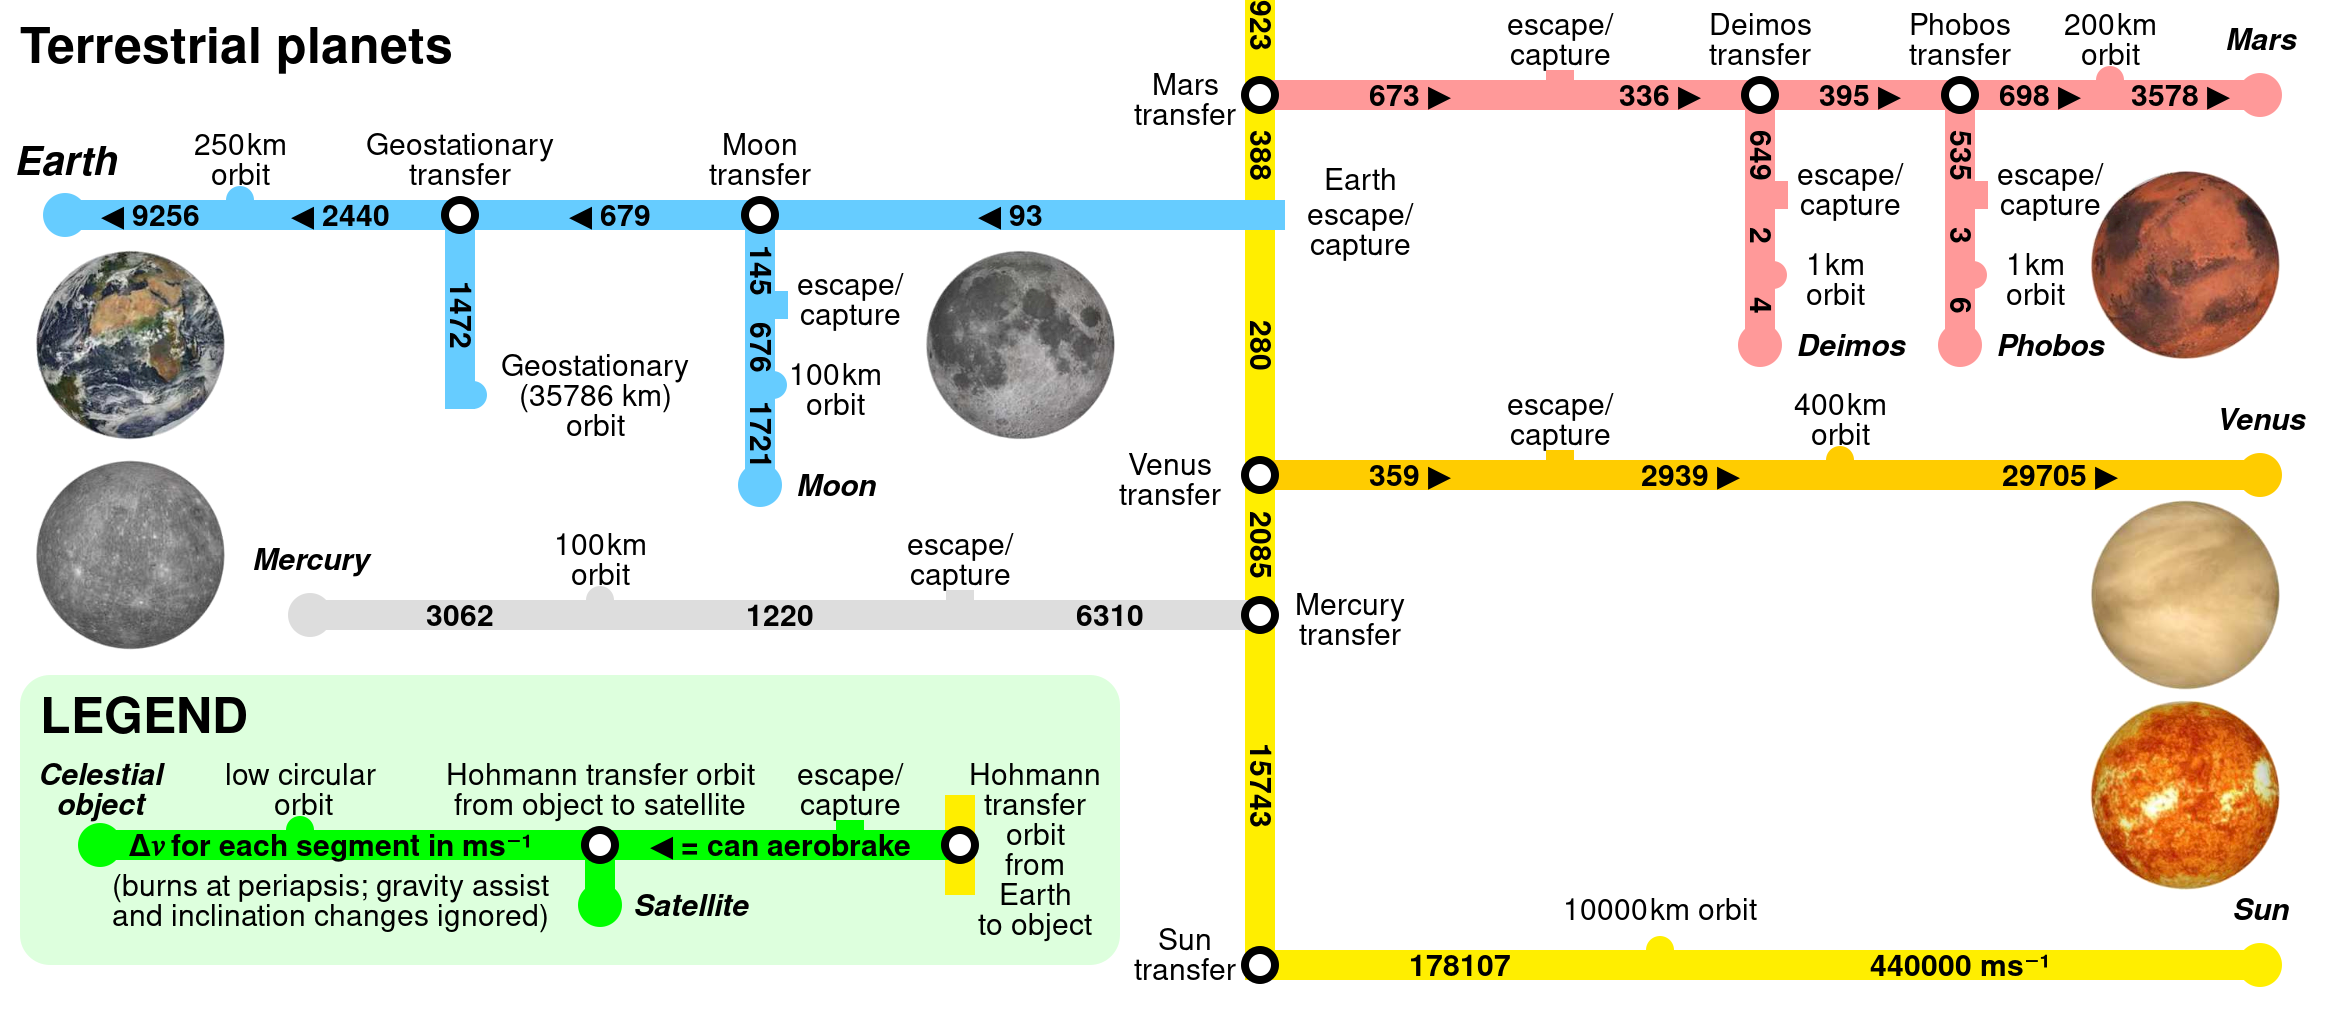
\includegraphics[scale=.2]{img/dv.png}
\caption{Delta-v map, assuming burns at periapsis, gravity assist, and ignoring inclination changes}
\end{figure}

For an Earth-Mars trip, a conservative estimate is located around $18000m.s^{-1}$, it is important to note that even though we could save up on fuel by using more efficient transfer techniques this would also come at the expanse of travel time, which, we will see, becomes a major hurdle of space travel. On the other hand aerobreaking is an option both on Earth and Mars and should be fully utilized to save up on fuel.
\newpage
\subsection{NTR}
Solid core nuclear thermal rockets, such as the NERVA-XE, make use of highly enriched U-235 fission reactor through which liquid hydrogen is passed serving as both coolant and propellant \cite{Finseth1991} as well as a good radiation shield.
\begin{figure}[hbtp]
\centering
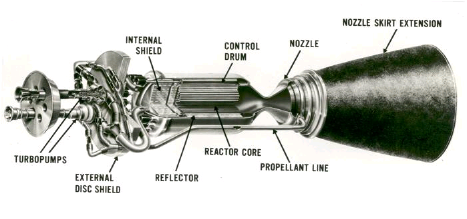
\includegraphics[scale=.7]{img/NERVA-solid-core-nuclear-propulsion-system.png}
\caption{NERVA solid core nuclear propulsion system. Source:
NASA.}
\end{figure}
%Liquid hydrogen is a propellant of choice due to its low molecular weight, which allows for high $I_{sp}$ as well as its low neutron absorbing cross section. Solid core design operate at around 2000°C which in conjunction with the use of hydrogen yield specific impulses approaching 1000s. The design is limited by the containment chamber's wall melting. Some newer design, such as gas core NTRs could yield specific impulses in the 3000s.


\section{Shielding}
Astronauts are exposed to higher doses of radiation in space mainly due to the lack of a magnetosphere and an atmosphere shielding them from SEP and GCR, the two main types of radiations in space. The dose grows stronger as one gets further away from the earth as its magnetosphere grows weaker the further away one gets from it.\\
The unprotected human body is quite weak to radiation, especially ionizing radiations and although the legislation is lacking for space workers the IAEA, specifies a dose of $20mSv$ per year averaged over five consecutive years (100 mSv in 5 years) and of $50mSv$ in any single year \cite{IAEA-GSG}, for occupational workers. A quantity well under was is proposed by \cite{Hoffman1997} as can be observed in figure 1.3.

\begin{figure}[hbtp]
\centering
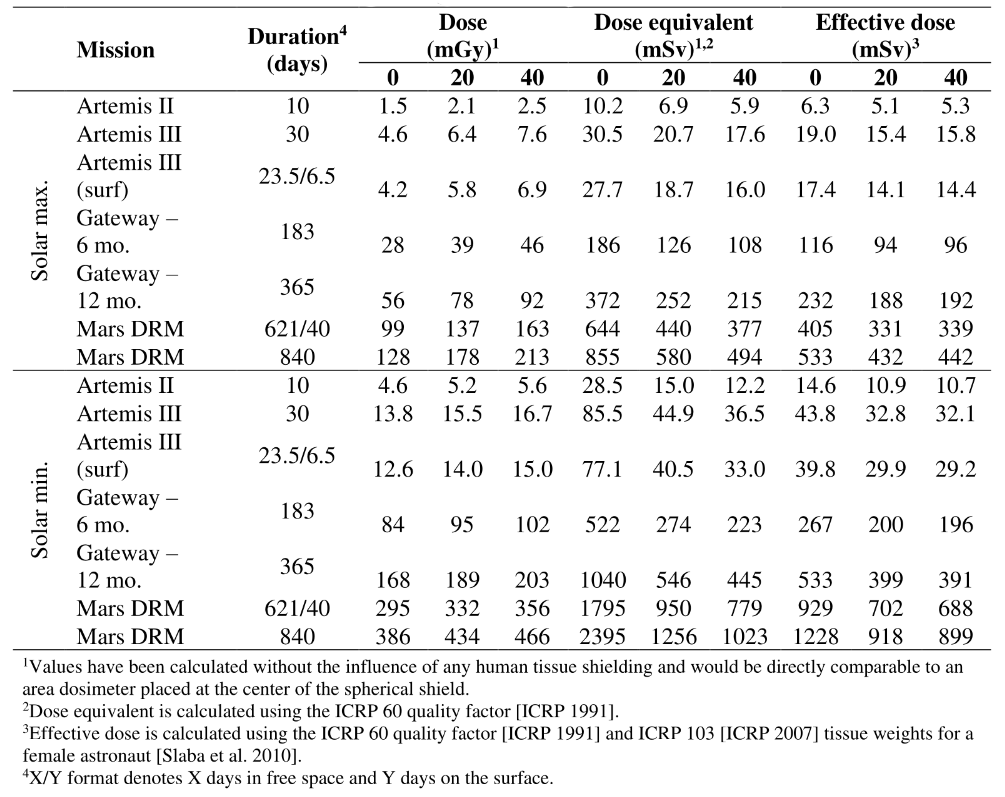
\includegraphics[scale=.5]{img/extrapo.png}
\caption{Mission Exposures derived by Scaling Daily Values from Figure 1.4 by Corresponding Mission Segment Durations, from \cite{Hoffman1997}}
\end{figure}

\begin{figure}[hbtp]
\centering
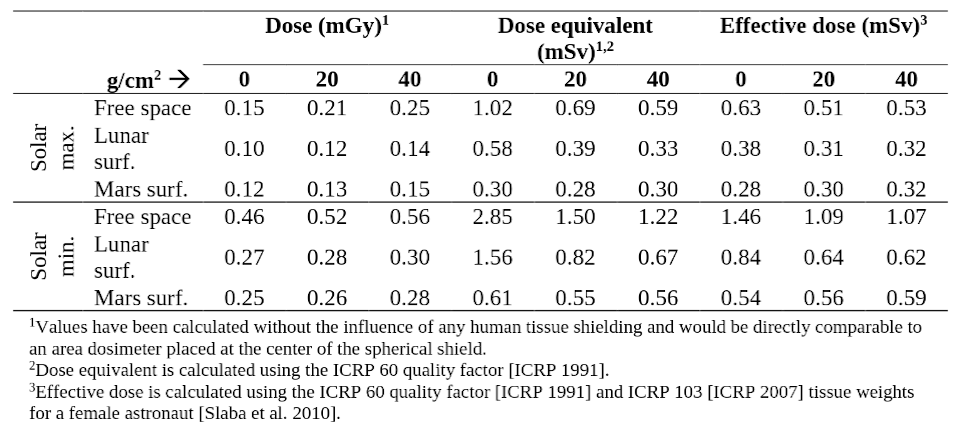
\includegraphics[scale=.5]{img/data.png}
\caption{Daily Exposure within 0, 20, and 40 g/cm2 Spherical Aluminum Shielding in Free Space and on Surface of Moon and Mars for Solar Minimum (2009) and Solar Maximum (2001) GCR Conditions, from \cite{Hoffman1997}}
\end{figure}

\newpage

\subsection{Radiation in Space}

\begin{figure}[hbtp]
\centering
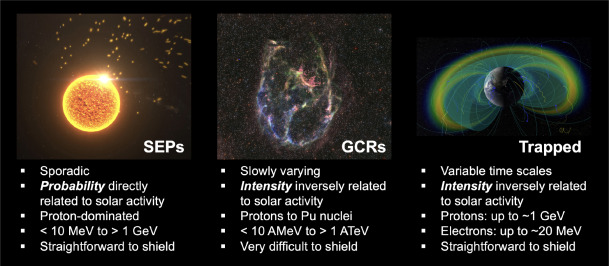
\includegraphics[scale=1]{img/Major characteristics of SEPs GCRs and trapped particle radiation.jpg}
\caption{Major characteristics of SEPs, GCRs, and trapped particle radiation. Images courtesy of NASA Scientific Visualization Studio. SEP image credit: NASA’s Goddard Space
Flight Center Conceptual Image Lab, GCR image credit: NASA/STScI/CXC/SAO, processing by Judy Schmidt, CC BY-NC-SA, Trapped image credit: NASA’s Scientific Visualization
Studio.}
\end{figure}




\begin{minipage}[b]{0.5\linewidth}
\centering
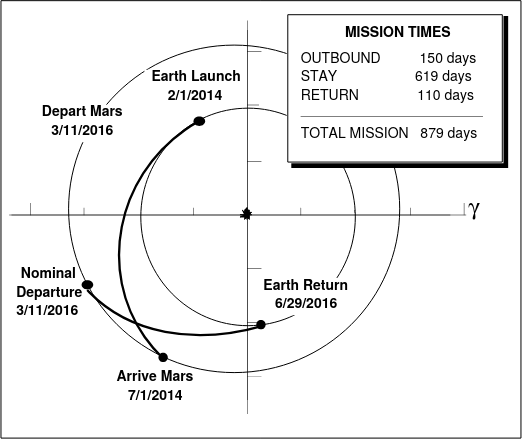
\includegraphics[scale=.4]{img/optimised traj.png}
\captionof{figure}{Typical fast-transit trajectory courtesy of \cite{Hoffman1997}}
\end{minipage} 
\hfill
\begin{minipage}[b]{0.35\linewidth}
In space, astronauts are exposed to three main kind of radiation environments, SEP, GCR and trapped radiations. For our purpose we will mainly focus on SEP and GCR radiations as the time spent around the earth and in the Van-Allen belt will be insignificant compared to the whole duration of the mission as highlighted in figure 1.6.
\end{minipage}

\newpage



\begin{minipage}[b]{0.3\linewidth}
\subsubsection{SEPs}
SEP are high energy charged particles originating in the solar atmosphere and transported by solar winds. They are mostly composed of high energy protons as reported in \cite{Jiggens2019}. Figure 1.7 shows the energy spectra from the 1989 solar event that resulted in a complete blackout of Hydro-Québec's power grid.
\end{minipage}
\hfill
\begin{minipage}[b]{0.6\linewidth}
\centering
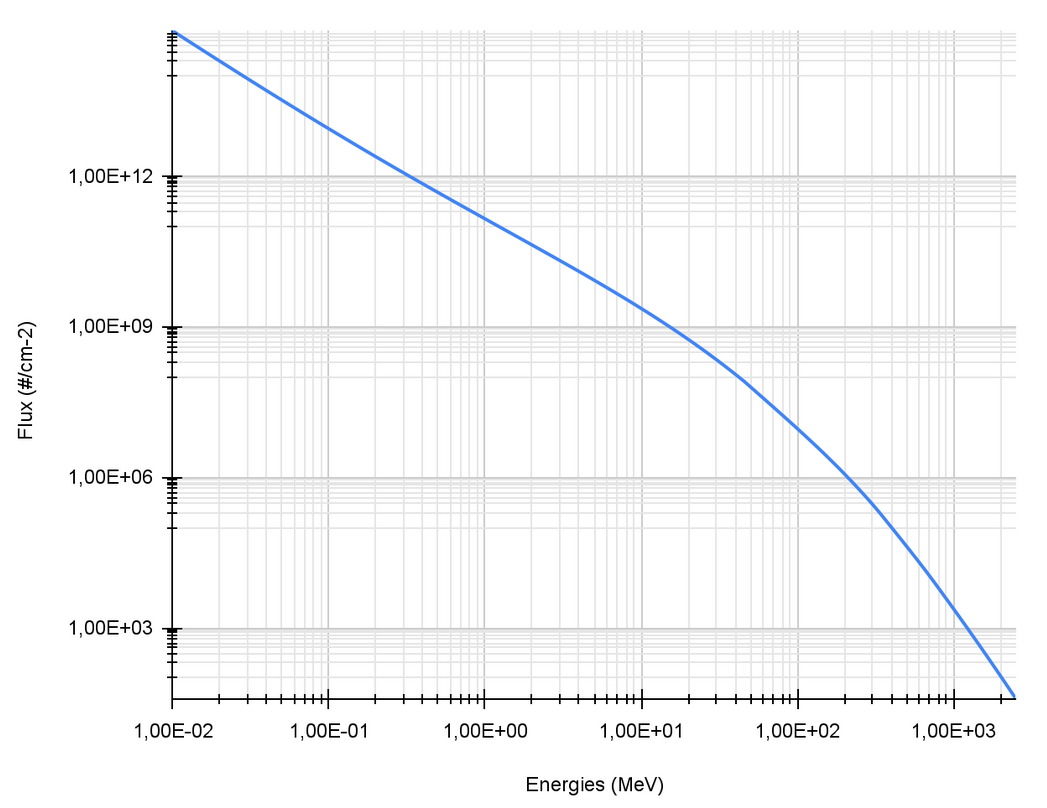
\includegraphics[scale=.3]{img/proton flux 1989.png}
\captionof{figure}{9-13th of March 1989 Solar storm}
\end{minipage} \\
\hfill\\



\begin{minipage}[b]{0.55\linewidth}
\centering
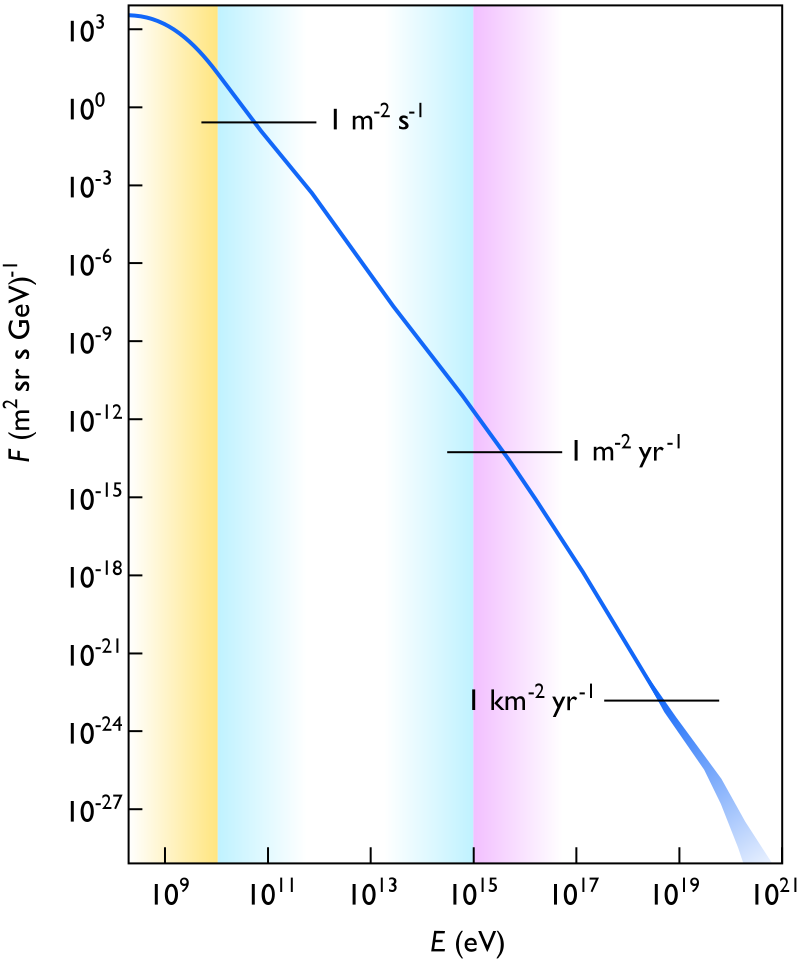
\includegraphics[scale=.25]{img/Cosmic_ray_flux_versus_particle_energy.svg.png}
\captionof{figure}{Cosmic flux versus particle energy at the top of Earth's atmosphere \cite{Sharma2008}}
\end{minipage}
\hfill
\begin{minipage}[b]{0.35\linewidth}
\subsubsection{GCRs}
CGR are high energy particles mostly composed of protons and HZE ions, some of them come from our sun but from our galaxy and other galaxies as well. The bulk of the flux is deflected to space by the heliosphere. Therefor, the solar cycle and thus the strength of the sun's magnetic sphere has a major influence on the influx of GCRs.
Solar maximums and minimums, the time where the sun's activity is respectively at its maximum and its minimum will play a big role in how we deal with GCRs.
\end{minipage}


\chapter{Results}
%provides raw (i.e., uninterpreted) data collected 	(perhaps) expresses the data in table form, as an easy-to-read figure, or as percentages/ratios

\section{Nuclear Propulsion}
\section{Shielding}


\chapter{Discussion}
% 	considers whether the data you obtained support the hypothesis 	explores the implications of your finding and judges the potential limitations of your experimental design


\chapter*{Acronyms}

\textbf{GCR: } Galactic Cosmic Ray\\
\textbf{SEP: } Solar Event Particles\\
\textbf{CEO: } Chief Executive Officer\\
\textbf{NTR: } Nuclear Thermal Rocket\\

\newpage


\bibliography{references}
\end{document}